\documentclass{exam}
\usepackage{amsfonts,amsmath,graphicx}
\newcommand*{\p}{\mathcal{P}}
\newcommand*{\QS}{\mathbb{Q}^*}
\setlength{\parskip}{6pt}

\title{Exercice 1 question 4 Concours général 2023}
\author{Romain Lemahieu}
\begin{document}
\maketitle
\section{Sujet}
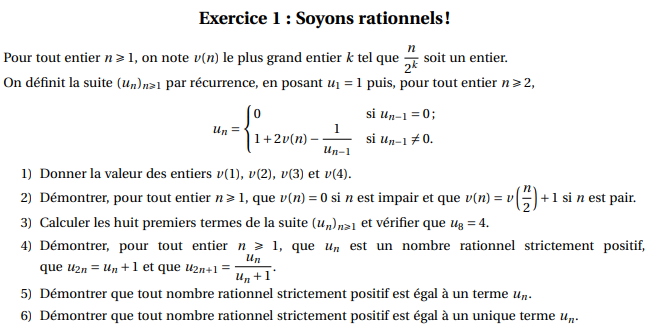
\includegraphics{sujet.png}
\section{Correction}
Soit 3 propriétés définis pour tout entiers naturels non nul :
\begin{align*}
\p_1(n)&:u_n \in \QS \\
\p_2(n)&:u_{2n}=u_n+1\\
\p_3(n)&:u_{2n+1}=\frac{u_n}{u_n+1}\\
\end{align*}
\pagebreak
\subsection{Initialisation}
Montrons que $\p_1(1)$ est vraie :
$$
u_1=1 
\quad 
1 \in \QS 
$$
Montrons que $\p_2(1)$ est vraie :
\begin{align*}
u_{2\times1}&=1+2\nu(2)-\frac{1}{u_{2\times1-1}}
&u_1+1=2
\\
u_2&=1+2\times1-\frac{1}{u_1}\\
u_2&=1+2\times1-\frac{1}{1}\\
u_2&=2
\end{align*}
Montrons que $\p_3(1)$ est vraie :
\begin{align*}
u_{2\times1+1}&=1+2\nu(3)-\frac{1}{u_{2\times1+1-1}}
&&
\frac{u_1}{u_1+1}=\frac{1}{1+1}
\\
u_3&=1-\frac{1}{u_2}
&&
\frac{u_1}{u_1+1}=\frac{1}{2}
\\
u_3&=1-\frac{1}{2}
\\
u_3&=\frac{1}{2}
\\
\end{align*}
\subsection{Hérédité}
En supposant que $\p_1(k)$, $\p_2(k)$ et $\p_3(k)$
sont vraie pour un certain entier $k$ naturel non nul
montrons que $\p_1(2k)$, $\p_1(2k+1)$, $\p_2(k+1)$ et $\p_3(k+1)$ le sont :

\subsubsection{Montrons que $\p_1$ est héréditaire}
Montrons que $\p_1(2k)$ est vraie supposant que $\p_1(k)$ et $\p_2(k)$ est vraie :
$$
u_k \in \QS \Rightarrow u_k+1 \in \QS \Rightarrow u_{2k}  \in \QS
$$
Montrons que $\p_1(2k+1)$ est vraie:
\begin{align*}
u_k& \in \QS
\\
\Rightarrow &u_k>0
\\
\Rightarrow &u_k+1>1
\\
\Rightarrow &\frac{1}{u_k+1}<1
\\
\Rightarrow &-1+\frac{1}{u_k+1}<0
&&
\text{Car la fonction $\frac{1}{x}$ est décroissante sur $\QS$}
\\
\Rightarrow &1-\frac{1}{u_k+1}>0
\\
\Rightarrow & \frac{u_k}{u_k+1}>0
\\
\Rightarrow & u_{2k+1}>0
&&
\text{En supposant que $\p_2(k)$ est vraie}
\\
\Rightarrow & u_{2k+1}  \in \QS
\\
\end{align*}
\subsubsection{Montrons que $\p_2$ est héréditaire}
\begin{align*}
u_{k+1}+1&=1+1+2\nu(k+1)-\frac{1}{u_k}
&&\text{En supposant que $\p_1(k)$ est vraie}
\\
u_{k+1}+1&=2+2(\nu(2k+2)-1)+1-\left(1+\frac{1}{u_k}\right)
&&\text{Car $2k+2$ est pair ssi $\nu(2k+2)=\nu(k+1)+1$}
\\
u_{k+1}+1&=1+2-2+2\nu(2k+2)-\frac{u_k+1}{u_k}\\
u_{k+1}+1&=1+2\nu(2k+2)-\frac{1}{u_{2k+1}}
&&\text{En supposant que $\p_3(k)$ et $\p_1(2k+1)$ sont vraies}
\\
u_{k+1}+1&=u_{2k+2}
\\
\end{align*}
\subsubsection{Montrons que $\p_3$ est héréditaire}
\begin{align*}
u_{2k+3}&=1+2\nu(2k+3)-\frac{1}{u_{2k+2}}
&&\text{En supposant que $\p_1(2k)$ est vraie}
\\
u_{2k+3}&=1-\frac{1}{u_{2k+2}}
&&\text{Car $2k+3$ est impair ssi $\nu(2k+3)=0$}
\\
u_{2k+3}&=1-\frac{1}{u_{k+1}+1}
&&\text{En supposant que $\p_2(k)$ est vraie}
\\
u_{2k+3}&=\frac{u_{k+1}+1-1}{u_{k+1}+1}
\\
u_{2k+3}&=\frac{u_{k+1}}{u_{k+1}+1}
\\
\end{align*}

\subsection{Conclusion}
Les propriétés $\p_1$, $\p_2$ et $\p_3$ étant initialisées et héréditaires donc :
$$
\forall n \in \mathbb{N}^*,
u_n \in \QS,
u_{2n}=u_n+1,
u_{2n+1}=\frac{u_n}{u_n+1}
$$
\end{document}